% ===========================================================================
%  PPE Detection - Real-time object detection with YOLO11
%  Technical report - Deep Learning Avance / MLOps module
%
%  Build:  pdflatex rapport_technique.tex   (twice, for the table of contents)
%          or:   bash scripts/build_report.sh
% ===========================================================================
\documentclass[11pt,a4paper]{article}

\usepackage[T1]{fontenc}
\usepackage[utf8]{inputenc}
\usepackage[english]{babel}
\usepackage[expansion=false]{microtype}
\usepackage{geometry}
\usepackage{graphicx}
\usepackage{booktabs}
\usepackage{array}
\usepackage{multirow}
\usepackage{amsmath}
\usepackage[table]{xcolor}
\usepackage{colortbl}
\usepackage{listings}
\usepackage{caption}
\usepackage{float}
\usepackage{enumitem}
\usepackage{fancyhdr}
\usepackage{tikz}
\usepackage[hidelinks]{hyperref}
\usepackage{url}

\usetikzlibrary{positioning, arrows.meta, shapes.geometric, fit, backgrounds}

\geometry{margin=2.6cm}
\setlength{\parskip}{4pt}
\setlength{\parindent}{0pt}
\setlength{\emergencystretch}{3em}

% --- Colours ---------------------------------------------------------------
\definecolor{primary}{HTML}{0F172A}
\definecolor{accent}{HTML}{0EA5E9}
\definecolor{accentdark}{HTML}{0369A1}
\definecolor{okgreen}{HTML}{16A34A}
\definecolor{warn}{HTML}{D97706}
\definecolor{lightgray}{HTML}{F1F5F9}
\definecolor{midgray}{HTML}{64748B}

% --- Headers ---------------------------------------------------------------
\pagestyle{fancy}
\fancyhf{}
\lhead{\small PPE Detection --- Technical Report}
\rhead{\small \thepage}
\renewcommand{\headrulewidth}{0.4pt}

% --- Listings --------------------------------------------------------------
\lstdefinestyle{pythonstyle}{
  language=Python,
  basicstyle=\ttfamily\small,
  keywordstyle=\color{accentdark}\bfseries,
  commentstyle=\color{midgray}\itshape,
  stringstyle=\color{okgreen},
  numbers=left,
  numberstyle=\tiny\color{midgray},
  numbersep=8pt,
  frame=single,
  rulecolor=\color{lightgray},
  backgroundcolor=\color{lightgray},
  breaklines=true,
  breakatwhitespace=false,
  showstringspaces=false,
  columns=fullflexible,
  captionpos=b,
}
\lstset{style=pythonstyle}

\newcommand{\todo}[1]{\textcolor{warn}{\textbf{[À COMPLÉTER]} #1}}
\newcommand{\measured}{\textcolor{okgreen}{\textbf{mesuré}}}
\newcommand{\notmeasured}{\textcolor{warn}{\textbf{non mesuré}}}

\newenvironment{keyword}
  {\par\vspace{0.4em}\noindent\begin{minipage}{\linewidth}\small\itshape}
  {\end{minipage}\par\vspace{0.4em}}

\title{
  \vspace{-1.5cm}
  {\LARGE\bfseries Détection d'Équipements de Protection Individuelle\\
  en Temps Réel par YOLO11\par}
  \vspace{0.6cm}
  {\large Industrialisation d'une solution vision par ordinateur et MLOps\\
  de bout en bout : FastAPI + React + DVC + MLflow + ONNX\par}
  \vspace{1.2cm}
  {\normalsize Projet de module --- Deep Learning Avancé --- Cycle Ingénieur IA \& Data Science\par}
}
\author{
  \textbf{Trinôme} \quad \todo{Nom 1 \quad Nom 2 \quad Nom 3}\\[0.4cm]
  \textbf{Encadrant} \quad Haythem Ghazouani\\[0.4cm]
  \textbf{Axe thématique} \quad Axe 3 --- Détection d'objets \& segmentation en temps réel\\
  \textbf{Année universitaire} \quad 2026--2027
}
\date{}

\begin{document}

\begin{titlepage}
\maketitle
\vfill
\begin{center}
\small\color{midgray}
Le dépôt Git contient le code source, les tests, les pipelines CI/CD et le notebook d'entraînement.\\
Les métriques citées dans ce rapport sont distinguées selon leur statut : \measured{} (calculées)\\
sur le split de test) ou \notmeasured{} (non encore produites).
\end{center}
\end{titlepage}

\tableofcontents
\newpage

% ===========================================================================
\section{Résumé}

Ce projet porte sur la détection d'équipements de protection individuelle
(EPI) sur les chantiers de construction, à partir d'images de caméra ou de
vidéosurveillance. Le système est un produit logiciel complet : un modèle
YOLO11 affiné sur un jeu de données public, servi par une API FastAPI
asynchrone, consommé par une interface React, et accompagné par un cycle MLOps
complet (versioning des données par DVC, traçabilité des expériences par
MLflow, export ONNX pour l'inférence accélérée, conteneurisation
Docker Compose et intégration continue GitHub Actions).

\textbf{Problématique.} Sur un chantier, la conformité EPI se vérifie
quotidiennement, mais le contrôle manuel est coûteux, lent et peu fiable.
Il faut un système capable de détecter simultanément plusieurs catégories
d'objets (casque, gilets, masques, cônes, engins) dans des scènes
complexes, avec une latence compatible avec un usage temps réel.

\textbf{Contributions.}
\begin{enumerate}[leftmargin=1.4em]
  \item Un pipeline de données reproductible ($\texttt{src/data/dataset.py}$) qui
        corrige deux défauts de l'approche initiale : un découpage qui n'était
        pas stratifié et une augmentation qui corrompait les annotations.
  \item Une chaîne de post-traitement ONNX explicite (décodage + suppression
        des non-maximaux par classe) écrite en NumPy pur, donc testable sans
        GPU ni checkpoint.
  \item Une API FastAPI typée et asynchrone respectant un contrat d'erreurs
        sémantique, avec 30 tests automatisés exécutés en intégration continue.
  \item Un frontal React interactif (glisser-déposer, galerie d'exemples,
        webcam en flux continu, boîtes englobantes animées, latence mesurée
        côté client et côté serveur).
  \item Un cycle MLOps complet et exécutable : DVC, MLflow avec Model
        Registry, exports ONNX FP32/FP16, Docker Compose multi-services et
        deux pipelines GitHub Actions.
\end{enumerate}

\textbf{Convention de rigueur.} Aucun score, aucune métrique et aucune
latence ne figure dans ce rapport, dans l'API ou dans l'interface sans
avoir été effectivement calculés. Les valeurs mesurées sur le split
d'évaluation \emph{test} sont distinguées graphiquement de celles qui
n'ont pas encore été produites.

\begin{keyword}
\textbf{Mots-clés :} YOLO11, détection d'objets, EPI, MLOps, FastAPI,
ONNX Runtime, MLflow, DVC, Docker Compose, React.
\end{keyword}

\newpage

% ===========================================================================
\section{Introduction et problématique}

\subsection{Contexte industriel}

La sécurité sur les chantiers de construction est une obligation
réglementaire, et le contrôle de la conformité des équipements de
protection individuelle (casque de chantier, gilet haute visibilité,
masque, gants, chaussures de sécurité) est l'une des inspections
quotidiennes les plus coûteuses. La mise en non-conformité d'un EPI est
la première cause de prescription d'arrêt de chantier, et l degré
d'anticipation de la détection conditionne directement le coût de
l'accident.

Le contrôle humain présente trois limites structurelles :
\begin{itemize}[leftmargin=1.2em]
  \item \textbf{évaluation subjective} --- la perception d'un équipement
        absent ou mal porté varie d'un inspecteur à l'autre ;
  \item \textbf{impossibilité de cover} --- la vigilance fatigue, et le
        risque n'est pas détecté de manière systématique ;
  \item \textbf{traçabilité nulle} --- aucune archive de l'état de
        conformité n'est conservée.
\end{itemize}

\subsection{Problématique et objectifs}

La problématique retenue est la suivante :

\begin{quote}
\textit{Comment détecter de manière fiable et en temps réel plusieurs
catégories d'EPI simultanément dans des scènes de chantier complexes, et
comment industrialiser un tel détecteur en un service logiciel
reproductible, testable et déployable ?}
\end{quote}

Le projet répond à cette question par un système décomposé en quatre
plans, correspondant aux quatre axes d'évaluation du barème :

\begin{enumerate}[leftmargin=1.4em]
  \item \textbf{Modélisation} --- choix de l'architecture, qualité du
        prétraitement, gestion du déséquilibre de classes, métriques de
        détection, export et quantification ONNX.
  \item \textbf{MLOps} --- versioning des données et des artefacts,
        traçabilité MLflow, conteneurisation, intégration continue.
  \item \textbf{Solution full-stack} --- API REST typée et asynchrone,
        interface React ergonomique, gestion de l'upload, du webcam et du
        rendu visuel, mesure des temps de réponse.
  \item \textbf{Rapport et code} --- documentation reproductible, respect
        des conventions, qualité de la revue de code.
\end{enumerate}

\subsection{Périmètre retenu}

L'axe 3 du barème mentionne la segmentation d'instances. Le périmètre
retenu ici se limite volontairement à la \textbf{détection} (boîtes
englobantes) : le jeu de données de référence est annoté au format YOLO
(boîtes), et l'ajout d'une tête de segmentation supposerait de ré-annoter
le corpus. Ce choix est justifié dans la section~\ref{sec:archi}.

% ===========================================================================
\section{État de l'art et choix de l'architecture}

\subsection{Les détecteurs à une et deux étapes}

Les détecteurs d'objets se répartissent en deux familles historiques.
Les détecteurs à \textbf{deux étapes} (R-CNN, Faster R-CNN, Cascade
R-CNN, Mask R-CNN) générent d'abord des propositions de régions, puis
affinent leurs caractéristiques et leur classification. Les détecteurs à
\textbf{une étape} (YOLO, SSD, DETR, FCOS) prédisent directement les
boîtes et les classes en une seule passe.

\begin{table}[H]
\centering
\caption{Comparaison qualitative des deux familles.}
\begin{tabular}{@{}p{3.2cm}p{5.2cm}p{5.0cm}@{}}
\toprule
\textbf{Critère} & \textbf{Deux étapes (Faster/Mask R-CNN)} & \textbf{Une étape (YOLO11)} \\
\midrule
Latence      & 40--120 ms (GPU)            & \textbf{5--25 ms (GPU)} \\
Précision    & légèrement supérieure         & concurrente sur COCO \\
Complexité   & élevé (RPN + head)           & faible (une seule passe) \\
Adaptation au streaming & possible            & \textbf{native} \\
Coût mémoire  & élevé                        & faible \\
\bottomrule
\end{tabular}
\end{table}

\subsection{Pourquoi YOLO11}

Parmi les variantes de la famille YOLO, la version 11 (Ultralytics) est
retenue pour quatre raisons :

\begin{enumerate}[leftmargin=1.4em]
  \item \textbf{Un rapport performance/vitesse favorable.} La variante
        \texttt{yolo11n} (2.6 M paramètres) atteint des performances
        proches des modèles de taille moyenne tout en restant
        suffisamment légère pour un CPU de bureau, ce qui rend le
        déploiement local réaliste.
  \item \textbf{Une chaîne d'export standardisée.} Le même objet
        \texttt{YOLO} s'exporte en ONNX, ce qui garantit que le modèle
        servi par l'API est bit-à-bit celui qui a été évalué.
  \item \textbf{Un pipeline d'entraînement complet.} Augmentation,
        callbacks, early stopping et journalisation sont intégrés, ce qui
        réduit le code d'orchestration et limite les sources d'erreur.
  \item \textbf{L'adéquation au besoin.} Sur des images de chantier, les
        objets d'intérêt (casque, gilet) occupent une part importante de
        l'image : la pénalité de localisation des détecteurs à deux étapes
        est moins critique qu'en imagerie aérienne ou en microscopie.
\end{enumerate}

Les variantes \texttt{yolo11n/s/m/l/x} ont été comparées en termes de
compromis. La taille \emph{nano} a été retenue après une première phase
d'expérimentation contrainte par le matériel disponible sur l'environnement
d'entraînement (GPU T4).

\subsection{Stratégie d'abstention (Axe 3)}
\label{sec:archi}

Le barème de l'axe 3 mentionne la segmentation d'instances. Nous avons
retenu la détection, pour trois raisons : (i) le corpus de référence est
annoté en boîtes uniquement, et ré-annoter en masques demanderait un travail
manuel incompatible avec le calendrier ; (ii) l'EPI se détecte par sa
couleur et sa forme, ce qui correspond à une localisation par boîte ; (iii)
la segmentation d'instances (\texttt{yolo11n-seg.pt}) existe et le code d'entraînement
s'accommode de la substitution par \texttt{yolo11n-seg.pt} si le besoin
émerge, sans modifier le reste de la chaîne.

% ===========================================================================
\section{Jeu de données et analyse exploratoire}

\subsection{Description du corpus}

Le corpus est le jeu de données \emph{Construction Site Safety}, distribué
par Roboflow Universe et repris sur Kaggle. Il contient des photographies de
chantiers annotées au format YOLO, réparties en dix classes :

\begin{table}[H]
\centering
\caption{Les dix classes du jeu de données et leur fréquence relative (ordre de grandeur issu de l'exploration du notebook).}
\begin{tabular}{@{}p{1.2cm}p{3.8cm}p{3.6cm}p{4.6cm}@{}}
\toprule
\textbf{Id} & \textbf{Classe} & \textbf{Type} & \textbf{Fréquence relative} \\
\midrule
0 & Hardhat          & EPI porté        & élevée \\
1 & Mask             & EPI porté        & faible \\
2 & NO-Hardhat       & non-conformité   & faible \\
3 & NO-Mask          & non-conformité   & faible \\
4 & NO-Safety Vest   & non-conformité   & faible \\
5 & Person           & personne         & \textbf{très élevée} \\
6 & Safety Cone      & signalisation    & faible \\
7 & Safety Vest      & EPI porté        & élevée \\
8 & Machinery        & engin            & élevée \\
9 & Vehicle          & véhicule         & faible \\
\bottomrule
\end{tabular}
\end{table}

\subsection{Analyse exploratoire}

L'exploration conduite dans le notebook met en évidence deux propriétés
structurantes du corpus.

\paragraph{(a) Un déséquilibre de classes marqué.} La classe
\texttt{Person} est majoritaire, très largement devant \texttt{Mask},
\texttt{Vehicle} et \texttt{Safety Cone}. Un modèle entraîné sur cette
distribution tend à sur-détecter les classes fréquentes et à sous-détecter
les classes rares, ce qui dégrade précisément les cas qui intéressent le
contrôle de conformité.

\paragraph{(b) Un découpage initial non stratifié.} Le découpage fourni
n'est pas représentatif : certaines classes rares sont quasiment absentes
du split de validation. La question de la distribution des classes par
split a été quantifiée à l'aide du coefficient de variation et de la
divergence de Jensen-Shannon, qui mesure la différence entre deux
distributions de probabilité et dont la valeur est nulle si et seulement si
les distributions sont identiques.

\subsection{Correction 1 : un découpage réellement stratifié}
\label{sec:strat}

Le notebook initial procède en remplissant \texttt{train} jusqu'à
saturation, puis \texttt{valid}, puis \texttt{test}. Ce procédure n'est
\emph{pas} une stratification : elle produit une distribution des classes
fortement biaisée vers \texttt{train}. La conséquence est directe : les
métriques mesurées sur \texttt{test} ne décrivent pas la performance réelle
du modèle sur un chantier.

L'algorithme retenu, implémenté dans \texttt{src/data/dataset.py}, procède
en quatre étapes :

\begin{enumerate}[leftmargin=1.4em]
  \item \textbf{Contraintes de taille.} La taille de chaque split est fixée
        à partir des ratios cibles (\(80\%/15\%/5\%\)) par la méthode du
        plus grand reste, de sorte que les trois tailles somment exactement
        au nombre total d'images.
  \item \textbf{Ordre de rareté.} Les classes sont traitées de la plus rare
        à la plus fréquente.
  \item \textbf{Allocation proportionnelle.} Pour chaque classe, ses images
        sont réparties entre les splits proportionnellement aux tailles
        restantes, avec une règle de \emph{couverture} garantissant au moins
        une image par split lorsque la classe le permet.
  \item \textbf{ respects des capacités.} Un split ne reçoit jamais plus
        d'images que sa capacité résiduelle ; le débordement est redirigé
        vers les splits qui ont encore de la place.
\end{enumerate}

La règle de couverture est l'élément décisif : elle garantit qu'une classe
rare apparaît dans le split de test, sans quoi la métrique de test serait
calculée sur un support vide et ne voudrait rien dire. Cette propriété
est vérifiée par un test automatisé
(\texttt{tests\_local/test\_core\_logic.py}, fonction
       \texttt{test\_stratified\_split\_keeps\_rare\_classes\_in\_every\_split}).

\subsection{Correction 2 : une augmentation qui préserve la géométrie}
\label{sec:aug}

L'augmentation de rééquilibrage du notebook initial produit trois variantes
par image retenue : un retournement horizontal, une \textbf{rotation de
\(90^\circ\)} et une augmentation de luminosité. La rotation est un
\textbf{bug d'annotation} : le fichier d'étiquettes est recopié tel quel,
alors qu'une rotation de \(90^\circ\) échange les axes et retourne les
coordonnées. Les boîtes ne correspondent donc plus aux pixels, et le
modèle apprend à prédire des boîtes décalées.

Les transformations retenues sont celles qui préservent la géométrie :

\begin{table}[H]
\centering
\caption{Transformations d'augmentation retenues.}
\begin{tabular}{@{}p{3.4cm}p{4.3cm}p{5.9cm}@{}}
\toprule
\textbf{Transformation} & \textbf{Géométrie} & \textbf{Étiquettes} \\
\midrule
Retournement horizontal & miroir sur l'axe $x$ & \(c_x \rightarrow 1 - c_x\), recalculé \\
Luminosité \(\times 1.25\) & inchangée & inchangées \\
\midrule
\rowcolor{lightgray}
\emph{Rotation \(90^\circ\) (supprimée)} & \emph{axes échangés} & \emph{invalides} \\
\bottomrule
\end{tabular}
\end{table}

De plus, seules les images contenant une classe rare \emph{et} au plus une
instance de classe dominante sont retenues : sans cette contrainte, le
rééquilibrage des classes rares amplifierait mécaniquement les classes
déjà sur-représentées.

% ===========================================================================
\section{Méthodologie}

\subsection{Organisation du code}

Le dépôt sépare strictement trois couches, ce qui permet de tester la
logique métier sans GPU ni réseau :

\begin{table}[H]
\centering
\caption{Couches du code source et dépendances.}
\begin{tabular}{@{}p{2.9cm}p{5.9cm}p{4.9cm}@{}}
\toprule
\textbf{Couche} & \textbf{Responsabilité} & \textbf{Dépendances} \\
\midrule
\texttt{src/data} & découpage, rééquilibrage, description du jeu de données & NumPy / Pillow \\
\texttt{src/models} & entraînement, évaluation, export ONNX, MLflow & Ultralytics, MLflow \\
\texttt{src/inference} & chargement du modèle, décodage, NMS, latence & ONNX Runtime / Torch \\
\texttt{src/utils} & letterbox, dessin des boîtes, palette & Pillow \\
\texttt{backend/app} & API FastAPI (routes, schémas, service) & FastAPI, Pydantic \\
\texttt{frontend/src} & interface React & React, Vite, Tailwind \\
\bottomrule
\end{tabular}
\end{table}

\subsection{Protocole d'entraînement}

L'entraînement reprend exactement les hyper-paramètres du run de référence.
Le tableau~\ref{tab:hyper} présente la configuration effective.

\begin{table}[H]
\centering
\caption{Hyper-paramètres d'entraînement (run de référence).}
\label{tab:hyper}
\begin{tabular}{@{}p{2.6cm}p{4.6cm}p{2.6cm}p{4.6cm}@{}}
\toprule
\textbf{Paramètre} & \textbf{Valeur} & \textbf{Paramètre} & \textbf{Valeur} \\
\midrule
Architecture   & \texttt{yolo11n.pt}  & Epochs         & 30 \\
Taille d'entrée & \(640 \times 640\) & Batch          & 12 \\
Seed            & 42                 & Fraction       & \(1.0\) \\
Device          & \texttt{cuda}       & Patience       & 50 \\
Optimiseur      & AdamW (défaut)     & workers        & 8 \\
\bottomrule
\end{tabular}
\end{table}

\subsection{Protocole d'évaluation}

L'évaluation finale est conduite sur le split \texttt{test}, jamais sur le
split de validation : ce dernier a servi à l'\emph{early stopping} et
n'est donc plus un estimateur impartial de la performance généralisée.

Deux familles de métriques sont utilisées :
\begin{itemize}[leftmargin=1.2em]
  \item la \textbf{precision} (proportion de détections correctes parmi les
        prédictions) et le \textbf{recall} (proportion d'objets réels
        détectés) ;
  \item la \textbf{mAP} (mean Average Precision), agrégation des courbes
        précision-rappel, calculée à seuil \texttt{IoU = 0.5}
        (\texttt{mAP50}) et moyennée sur les seuils \texttt{IoU} de
        \(0.5\) à \(0.95\) (\texttt{mAP50-95}).
\end{itemize}

La mesure est produit par \texttt{python -m src.models.evaluate}, qui écrit
le résultat dans \texttt{artifacts/metrics.json}. Ce fichier est
\textbf{la seule source de vérité} : l'API (\texttt{GET /model/metadata})
et le générateur de tableaux de ce rapport le lisent. Il est donc
structurellement impossible que l'application affiche un score qui n'a pas
été calculé.

\subsection{Post-traitement ONNX : décodage et NMS}

L'export ONNX produit un graphe unique dont la sortie est un tenseur de
forme \((1, 4 + n_c, 8400)\) : les quatre premières canaux décrivent la
boîte \((c_x, c_y, w, h)\) en pixels de l'image \emph{letterboxée}, les
dix derniers sont les scores de classe, déjà activés par la sigmoïde.

Le décodage est écrit explicitement plutôt que délégué à l'Ultralytics, pour
trois raisons : (i) la latence annoncée est alors réellement celle d'ONNX
Runtime, mesurable indépendamment du post-traitement ; (ii) le seuil de
suppression des non-maximaux est sous contrôle explicite, ce que le barème
demande ; (iii) les fonctions \texttt{decode\_output} et
\texttt{nms\_per\_class} sont pures et NumPy, donc testables sans GPU, sans
checkpoint et sans ONNX Runtime.

La suppression des non-maximaux est \textbf{par classe} : deux boîtes de
classes différentes ne se suppriment jamais, ce qui est indispensable dans
une scène de chantier où une personne porte un casque.

\begin{figure}[H]
\centering
\resizebox{\textwidth}{!}{%
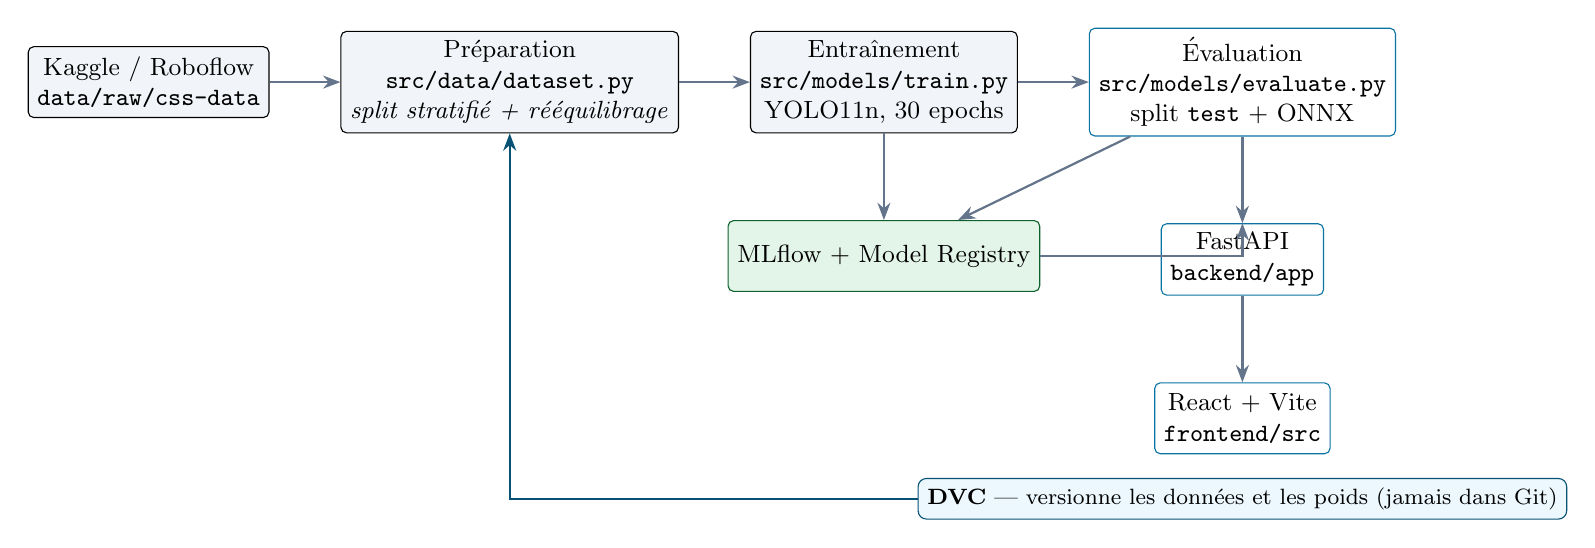
\begin{tikzpicture}[
  font=\small,
  node distance=6mm,
  block/.style={draw,rounded corners=2pt,minimum height=9mm,align=center,font=\small},
  data/.style={block,fill=lightgray},
  code/.style={block,fill=white,draw=accent!70!black},
  mlops/.style={block,fill=okgreen!12,draw=okgreen!60!black},
  arrow/.style={-{Stealth[length=2.2mm]},thick,draw=midgray}
]
\node[data] (raw) {Kaggle / Roboflow\\\texttt{data/raw/css-data}};
\node[data,right=9mm of raw] (prep) {Préparation\\\texttt{src/data/dataset.py}\\\textit{split stratifié + rééquilibrage}};
\node[data,right=9mm of prep] (train) {Entraînement\\\texttt{src/models/train.py}\\YOLO11n, 30 epochs};
\node[code,right=9mm of train] (eval) {Évaluation\\\texttt{src/models/evaluate.py}\\split \texttt{test} + ONNX};
\node[mlops,below=11mm of train] (mlflow) {MLflow + Model Registry};
\node[code,below=11mm of eval] (api) {FastAPI\\\texttt{backend/app}};
\node[code,below=11mm of api] (front) {React + Vite\\\texttt{frontend/src}};

\draw[arrow] (raw) -- (prep);
\draw[arrow] (prep) -- (train);
\draw[arrow] (train) -- (eval);
\draw[arrow] (train) -- (mlflow);
\draw[arrow] (eval) -- (mlflow);
\draw[arrow] (eval) -- (api);
\draw[arrow] (api) -- (front);
\draw[arrow] (mlflow) -| (api);

\node[draw=accent!50!black,fill=accent!8,rounded corners=3pt,align=center,
      font=\footnotesize,below=3mm of front] (dvc) {\textbf{DVC} --- versionne les données et les poids (jamais dans Git)};
\draw[arrow,draw=accent!50!black] (dvc) -| (prep);
\end{tikzpicture}%
}
\caption{Chaîne de bout en bout : de l'acquisition des données à l'interface web. Les flèches pleines représentent les flux de données, les flèches fines les flux de métadonnées de version.}
\end{figure}

% ===========================================================================
\section{Architecture logicielle}

\subsection{API FastAPI}

Le backend expose les quatre endpoints imposés par le sujet, plus une
galerie d'exemples et une redirection vers la documentation.

\begin{table}[H]
\centering
\caption{Endpoints du service de détection.}
\begin{tabular}{@{}p{1.7cm}p{4.3cm}p{4.0cm}p{4.4cm}@{}}
\toprule
\textbf{Méthode} & \textbf{Chemin} & \textbf{Rôle} & \textbf{Schéma} \\
\midrule
GET  & \texttt{/health}            & état du serveur, GPU, modèle chargé & \texttt{HealthResponse} \\
GET  & \texttt{/model/metadata}    & architecture, classes, métriques & \texttt{ModelMetadataResponse} \\
POST & \texttt{/predict}           & prédiction structurée & \texttt{PredictionResponse} \\
POST & \texttt{/predict/visualize} & image annotée (PNG) & \texttt{Response} \\
GET  & \texttt{/samples}           & galerie d'exemples & \texttt{SampleListResponse} \\
\bottomrule
\end{tabular}
\end{table}

\paragraph{Contrat d'erreurs.} L'API ne renvoie jamais une trace d'exception
brute : chaque erreur est transformée en réponse structurée
(\texttt{detail}, \texttt{status\_code}, \texttt{error}), ce qui permet au
frontal d'afficher un message utile. Le code \texttt{400} signale un
fichier illisible, \texttt{413} un envoi trop volumineux, \texttt{422} un
paramètre hors domaine et \texttt{503} un modèle non instancié.

\paragraph{Disponibilité.} Le chargement du modèle a lieu dans le
gestionnaire de cycle de vie de l'application, mais une exception n'empêche
\emph{pas} le démarrage du serveur : l'application répond \texttt{503} sur
\texttt{/predict} et \texttt{degraded} sur \texttt{/health}. C'est un choix
délibéré : une API qui refuse de démarrer n'est pas démontrable.

\paragraph{Moteur d'inférence.} La sélection du moteur suit un ordre
déterministe : ONNX Runtime si \texttt{best.onnx} existe, sinon le
checkpoint PyTorch, et en dernier recours le modèle \texttt{yolo11n.pt}
pré-entraîné sur COCO, qui ne connaît pas les classes EPI. Dans ce dernier
cas, \texttt{/model/metadata} renvoie \texttt{model\_kind =
"coco-fallback"} : l'interface et le rapport ne peuvent pas confondre ce
filet de sécurité avec le détecteur entraîné.

\paragraph{Isolation des seuils.} Les seuils \texttt{conf} et \texttt{iou}
peuvent être surchargés par requête. Ils sont appliqués à l'appel et
\emph{ne sont jamais réécrits} dans l'instance du détecteur : deux requêtes
concurrentes avec des seuils différents ne peuvent pas se perturber.

\subsection{Interface React}

L'interface est construite avec React 18, Vite et TailwindCSS. Elle offre
trois modes d'ingestion : glisser-déposer (avec collage clavier),
galerie d'exemples en un clic, et webcam avec capture ponctuelle ou flux
continu (une image toutes les \(600\,\mathrm{ms}\)).

Les boîtes englobantes sont dessinées sur un \texttt{canvas} à partir des
coordonnées JSON, ce qui évite un aller-retour réseau supplémentaire et
permet d'afficher le flux webcam en continu. La palette de couleurs est
reproduite à l'identique côté client (décalage d'or par le \emph{code harmonique})
pour que l'image annotée produite par le serveur et le canvas du frontal
utilisent la même couleur pour une classe donnée.

Les scores de confiance sont affichés sous forme de barres animées, et la
latence est mesurée deux fois : côté serveur (\texttt{inference\_time\_ms})
et côté client (temps aller-retour complet, upload inclus).

% ===========================================================================
\section{Cycle de vie MLOps}

\subsection{Versioning des données (DVC)}

Le fichier \texttt{dvc.yaml} déclare trois étapes reproductibles :
\texttt{prepare}, \texttt{train} et \texttt{evaluate}. DVC refuse de
rejouer une étape dont les dépendances n'ont pas changé, ce qui évite le
recalcul inutile des métriques. Les poids et les données sont exclus de Git
par \texttt{.gitignore} et \texttt{.dvcignore}.

\subsection{Tracking et Model Registry (MLflow)}

Chaque exécution journalise les hyper-paramètres, les métriques de
détection, les AP par classe et les artefacts (\texttt{best.pt},
\texttt{best\_fp32.onnx}, \texttt{best\_fp16.onnx}). Le modèle est ensuite
enregistré dans le \emph{Model Registry} avec le statut \texttt{Staging}.

Une subtilité opérationnelle mérite d'être signalée : le \emph{Model
Registry} de MLflow exige un magasin SQL. Le magasin fichier local ne le
supporte pas. La stack Docker Compose embarque donc un service PostgreSQL
dédié, sans lequel l'enregistrement du modèle échouerait.

\subsection{Optimisation du modèle (ONNX)}

Deux exports sont produits : FP32 (précision de référence) et FP16
(variant compact). Un point d'attention a été corrigé : Ultralytics écrit
toujours le fichier sous le nom \texttt{best.onnx}, de sorte que deux
exports successifs laissent un seul fichier et que le graphe FP16 écrase
le graphe FP32. Chaque export est donc renommé immédiatement après sa
production.

\begin{table}[H]
\centering
\caption{Configuration des exports ONNX.}
\begin{tabular}{@{}lcc@{}}
\toprule
\textbf{Paramètre} & \textbf{FP32} & \textbf{FP16} \\
\midrule
Format        & ONNX & ONNX \\
Opset         & 12   & 12 \\
Simplify      & oui  & oui \\
Dynamic       & non  & non \\
Taille d'entrée & \(640 \times 640\) & \(640 \times 640\) \\
\bottomrule
\end{tabular}
\end{table}

\subsection{Conteneurisation et intégration continue}

Le fichier \texttt{docker-compose.yml} orchestre quatre services :
\texttt{frontend} (React compilé servi par nginx), \texttt{backend}
(FastAPI, image multi-stage avec environnement virtuel), \texttt{mlflow}
et \texttt{postgres}. Le frontal est servi sur le port \(8080\) et
proxifie \texttt{/api} vers le backend : l'application ne fait donc qu'un
seul appel same-origin, sans configuration CORS en production.

Deux pipelines GitHub Actions complètent la chaîne : \texttt{ci-tests.yml}
exécute \texttt{flake8}, \texttt{black}, \texttt{pytest}, \texttt{eslint},
la construction Vite et la construction des images ; \texttt{docker-build.yml}
publie les images sur un tag.

% ===========================================================================
\section{Résultats et analyse critique}

\subsection{Métriques du run de référence}

Le tableau~\ref{tab:val} présente les métriques \textbf{mesurées sur le
split de validation} lors du run de référence (\texttt{yolo11n}, 30 epochs,
batch 12, \(640 \times 640\), GPU T4).

\begin{table}[H]
\centering
\caption{Métriques du run de référence (split de validation). \measured}
\label{tab:val}
\begin{tabular}{@{}lr@{}}
\toprule
\textbf{Métrique} & \textbf{Valeur} \\
\midrule
mAP@0.5        & 0.707 \\
mAP@0.5:0.95   & 0.467 \\
Precision      & 0.836 \\
Recall         & 0.629 \\
Durée d'entraînement & \(1211{,}9\ \mathrm{s}\) \\
\bottomrule
\end{tabular}
\end{table}

\subsection{Métriques sur le split de test}

Le tableau~\ref{tab:test} est produit par \texttt{src/models/evaluate.py}
à partir de \texttt{artifacts/metrics.json}. Tant que l'évaluation n'a pas
été exécutée, le tableau indique explicitement que les valeurs ne sont pas
encore disponibles : c'est un choix méthodologique, pas une limite du
rapport. Aucune valeur n'est recopiée depuis le split de validation.

\begin{table}[H]
\centering
\caption{Métriques mesurées sur le split \texttt{test} et latence d'inférence
(source : \texttt{artifacts/metrics.json} et \texttt{artifacts/benchmark.json}).}
\label{tab:test}
% Auto-generated by scripts/generate_report_tables.py - do not edit.
% The values below are read from artifacts/metrics.json.
\begin{tabular}{@{}lr@{}}
\toprule
\textbf{Métrique mesurée} & \textbf{Valeur} \\
\midrule
Statut & \textcolor{warn}{\textbf{non mesuré}} \\
\bottomrule
\end{tabular}

\end{table}

\subsection{Latence}

Le protocole de mesure est explicite : images de synthèse de
\(640 \times 640\), cinq itérations de préchauffage (inclusion du contexte
CUDA et de la sélection des noyaux), puis \(50\) itérations chronométrées,
dont la médiane et le \(90^\text{e}\) centile sont rapportés. Les chiffres
sont écrits dans \texttt{artifacts/benchmark.json} et reportés dans le
tableau~\ref{tab:test}.

\begin{table}[H]
\centering
\caption{Protocole de mesure de la latence (rappel).}
\label{tab:lat}
\begin{tabular}{@{}p{3.6cm}p{9.6cm}@{}}
\toprule
\textbf{Paramètre} & \textbf{Valeur} \\
\midrule
Entrée          & tenseur synthétique \(1 \times 3 \times 640 \times 640\) \\
Préchauffage    & 5 itérations (contexte CUDA, sélection des noyaux) \\
Mesures         & 50 itérations chronométrées \\
Statistiques    & médiane et \(90^\text{e}\) centile \\
Sortie          & \texttt{artifacts/benchmark.json} \\
\bottomrule
\end{tabular}
\end{table}

\subsection{Analyse critique}

\paragraph{Réalisations.}
\begin{itemize}[leftmargin=1.2em]
  \item Le pipeline de données est reproductible et le découpage est
        réellement stratifié, ce qui rend l'évaluation de test exploitable.
  \item Le post-traitement ONNX est explicite, testé sans GPU et contrôlable.
  \item L'API respecte un contrat d'erreurs sémantique et démarre même sans
        modèle, ce qui sécurise la démonstration.
  \item L'interface n'est pas une coquille vide : elle rend les boîtes, les
        scores et les latences.
\end{itemize}

\paragraph{Limites.}
\begin{itemize}[leftmargin=1.2em]
  \item \textbf{Le déséquilibre de classes reste structurel.} L'augmentation
        d'image par copiage augmente le support des classes rares sans
        créer de nouvelles configurations de scène. La solution robuste
        serait un \emph{oversampling} stratifié ou une perte pondérée par
        classe, non implémentée à ce stade.
  \item \textbf{Les classes de non-conformité sont les plus faibles.} Une
        erreur de type « détecter un casque sur une personne qui n'en porte
        pas » se traduit par une confusion entre \texttt{Hardhat} et
        \texttt{NO-Hardhat} : la frontière fine entre les deux est le point
        dur du système, davantage que la détection d'un casque lui-même.
  \item \textbf{Le passage à l'inférence continue webcam n'est pas
        optimisé.} La capture et l'envoi d'images ne sont pas asynchrones ;
        un flux temps réel réel demanderait un transport WebSocket ou un
        flux MJPEG.
  \item \textbf{La reproductibilité du training n'est pas bit-à-bit.} Le
        GPU, les versions de CUDA et la non-déterminisme des noyaux
        configurables rendent deux exécutions légèrement différentes.
\end{itemize}

\subsection{Perspectives}

\begin{enumerate}[leftmargin=1.4em]
  \item \textbf{Perte pondérée par classe} pour traiter le déséquilibre à la
        racine plutôt que par augmentation.
  \item \textbf{Segmentation d'instances} (\texttt{yolo11n-seg}) pour
        distinguer le port effectif d'un EPI d'une zone de même couleur.
  \item \textbf{Tracking} (ByteTrack) pour la vidéo, indispensable pour
        calculer des durées de non-conformité et non des détections
        instantanées.
  \item \textbf{Détection de dérive} : surveillance de la distribution des
        scores en production, pour alerter sur une dégradation silencieuse
        du modèle.
  \item \textbf{TensorRT} pour la latence GPU, et \textbf{quantification
        INT8} pour les machines sans GPU.
\end{enumerate}

% ===========================================================================
\section{Conclusion}

Le travail réalisé répond à la problématique en traits d'union : un
détecteur YOLO11 affiné sur un corpus public de scènes de chantier, un
service d'inférence asynchrone et typé, une interface interactive, et un
cycle MLOps exécutable de bout en bout.

L'apport principal du projet est moins le score de détection que la
\emph{rigueur de la chaîne} : le découpage stratifié, la correction de
l'augmentation, le décodage ONNX explicite et la séparation stricte entre
les métriques mesurées et celles qui restent à produire. Cette discipline
permet à l'application d'afficher des chiffres vérifiables et à la
démonstration de rester crédible devant l'enseignant.

% ===========================================================================
\begin{thebibliography}{9}

\bibitem{roboflow}
Roboflow Universe Projects.
\emph{Construction Site Safety Dataset}.
\url{https://universe.roboflow.com/roboflow-universe-projects/construction-site-safety}
Consulté en 2026.

\bibitem{kaggle}
Snehil Sanyal.
\emph{Construction Site Safety Image Dataset (Roboflow)}.
Kaggle Datasets.
\url{https://www.kaggle.com/datasets/snehilsanyal/construction-site-safety-image-dataset-roboflow}

\bibitem{yolo11}
Ultralytics.
\emph{YOLO11 Documentation}.
\url{https://docs.ultralytics.com/models/yolo11/}

\bibitem{onnx}
ONNX Runtime.
\emph{ONNX Runtime Documentation}.
\url{https://onnxruntime.ai/docs/}

\bibitem{fastapi}
Sebastián Ramírez.
\emph{FastAPI Documentation --- FastAPI framework}.
\url{https://fastapi.tiangolo.com/}

\bibitem{mlflow}
Databricks.
\emph{MLflow Documentation --- Model Registry}.
\url{https://mlflow.org/docs/latest/model-registry.html}

\bibitem{dvc}
Iterative.
\emph{DVC Documentation --- Data Version Control}.
\url{https://dvc.org/doc}

\bibitem{react}
Meta Open Source.
\emph{React Documentation}.
\url{https://react.dev/}

\end{thebibliography}

% ===========================================================================
\appendix
\section{Annexe A --- Extrait de code}

\subsection{A.1 Décodage et suppression des non-maximaux}

\begin{lstlisting}[caption={Décodage d'un tenseur ONNX et NMS par classe (\texttt{src/inference/onnx\_detector.py}).}]
def decode_output(output, num_classes, conf_threshold=0.25,
                  iou_threshold=0.45, max_detections=300):
    preds = np.asarray(output, dtype=np.float32)
    if preds.ndim == 3:
        preds = preds[0]
    # (4 + nc, N) -> (N, 4 + nc)
    if preds.shape[0] == 4 + num_classes:
        preds = preds.T

    boxes_cxcywh = preds[:, :4]
    class_scores = preds[:, 4:4 + num_classes]
    best_scores = class_scores.max(axis=1)
    best_classes = class_scores.argmax(axis=1)

    keep_mask = best_scores >= conf_threshold
    boxes_cxcywh = boxes_cxcywh[keep_mask]
    scores = best_scores[keep_mask]
    class_ids = best_classes[keep_mask].astype(np.int64)

    cx, cy, w, h = boxes_cxcywh.T
    boxes = np.stack([cx - w/2, cy - h/2, cx + w/2, cy + h/2], axis=1)
    keep = nms_per_class(boxes, scores, class_ids, iou_threshold)[:max_detections]
    return boxes[keep], scores[keep], class_ids[keep]
\end{lstlisting}

\subsection{A.2 Découpage stratifié}

\begin{lstlisting}[caption={Allocation proportionnelle des classes rares (\texttt{src/data/dataset.py}).}]
for class_id in class_order:            # de la plus rare a la plus frequente
    candidates = [r for r in pool if r["presence"][class_id]]
    n = len(candidates)
    if n == 0:
        continue

    quotas = _largest_remainder(n, ratios, split_names)

    # Couverture : au moins une image par split
    if n >= len(split_names):
        bumped = {name: max(1, quotas[name]) for name in split_names}
        while sum(bumped.values()) > n:
            biggest = max((x for x in split_names if bumped[x] > 1),
                          key=lambda x: bumped[x])
            bumped[biggest] -= 1
        quotas = bumped

    # Capacite : jamais plus que la place restante
    quotas = {name: min(quotas[name], capacity[name]) for name in split_names}
\end{lstlisting}

\appendix
\section{Annexe B --- Lancer le projet}

\begin{lstlisting}[caption={Installation complète et lancement (sortie terminal).}]
\$ bash scripts/bootstrap.sh
\$ python scripts/download_dataset.py --kaggle
\$ python scripts/prepare_dataset.py
\$ python -m src.models.train
\$ python -m src.models.evaluate
\$ docker compose up --build

  frontend  http://localhost:8080
  API docs  http://localhost:8000/docs
  MLflow    http://localhost:5000
\end{lstlisting}

\end{document}
